%%%%%%%%%%%%%%%%%%%%%%%%%%%%%%%%%%%%%%%%%%%%%%%%%%%%%%%%%%%%%%%%%
\chapter{KULLANILAN TEKNOLOJİLER}\label{ch:fp}
%%%%%%%%%%%%%%%%%%%%%%%%%%%%%%%%%%%%%%%%%%%%%%%%%%%%%%%%%%%%%%%%%
\vspace*{-1cm}
Bu bölümde Öğrenci İşleri uygulamasını yaparken kullanacak olduğum teknolojilerden söz edeceğim.

\section{React}
React, kullanıcı arayüzü (UI) oluşturmak için kullanılan en popüler JavaScript kütüphanesidir. Web siteleri işlemek için kullanıcı çıktısına harika yanıt sunan bir yöntemi kullanır.

Bu aracın bileşenleri Facebook tarafından geliştirilmiştir. 2013’de açık kaynaklı bir JavaScript olarak piyasaya sürülmüştür.

React'ı Öğrenci İşleri projesinde web uygulamasındaki frontend alanları için kullanacağım.

\begin{figure} [h]
 \centering
 
\includegraphics[width=120pt,keepaspectratio=true]{./fig/React}
  \caption{React}
 \label{fig:ch3-1}
\end{figure}

\section{React Native}

React Native, açık kaynaklı bir UI yazılım çerçevesidir.React Native tek bir dil üzerinden kodlama yapabilme ve geliştirilen uygulamanın bir çok platformda çalşma olanağı sunar.

React Native'i Öğrenci İşleri projesinde mobil uygulamasındaki frontend alanları için kullanacağım.

\begin{figure} [h]
 \centering
 
\includegraphics[width=82pt,keepaspectratio=true]{./fig/react-native}
  \caption{React Native}
 \label{fig:ch3-2}
\end{figure}

\section{Firebase}
Firebase, Google tarafından mobil ve web uygulamaları oluşturmak için geliştirilmiş ücretsiz bir platformdur.

Kullanıcı girişlerinin olduğu ve verilerin saklandığı birden fazla platformda geliştirilecek bir yazılım projeniz varsa Firebase size bu konuda oldukça fayda sağlayacaktır.2022 itibariyle bulut bilişim teknolojisinin gelişmesiyle birlikte, büyük verilerin internet üzerinde depolanabilirliği ve erişilebilirliği kolaylaşmıştır.

Firebase'i Öğrenci İşleri projesinde hem web hem de mobil uygulamadaki backend alanları için kullanacağım.

\begin{figure} [h]
 \centering
 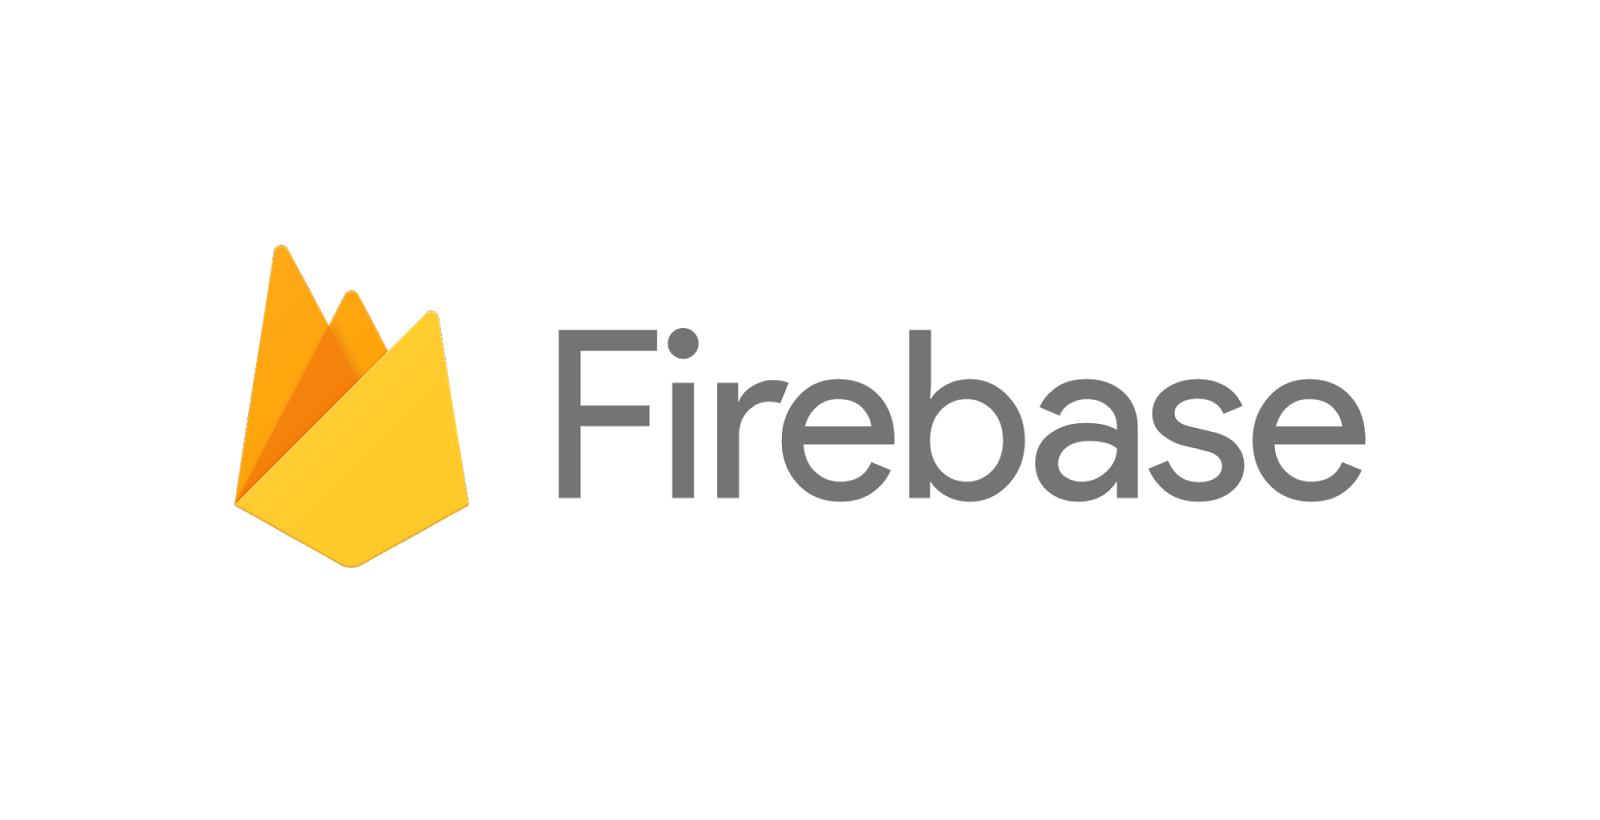
\includegraphics[width=180pt,keepaspectratio=true]{./fig/Firebase}
  \caption{Firebase}
 \label{fig:ch3-3}
\end{figure}